\section{Two level system evolution\label{sec:firstLecture}}
To represent a qubit state, we use a Bloch sphere, and say that

\begin{equation}
  \label{eqn:bloch}
  \ket{\psi} = \begin{cases}
    \cos\left(\frac{\theta}{2}\right)\ket{0} + e^{i\phi}\sin\left(\frac{\theta}{2}\right)\ket{1}\\
    \alpha\ket{0}+\beta\ket{1}
  \end{cases},
\end{equation}

\noindent from which we can express

   \begin{equation}
     \left\lbrace\begin{aligned}
         \alpha & = \cos\left(\frac{\theta}{2}\right)\\
         \beta & = e^{i\phi}\sin\left(\frac{\theta}{2}\right)
       \end{aligned}\right. \Rightarrow
     \left\lbrace\begin{aligned}
         \left|\frac{\beta}{\alpha}\right| & =\tan\left(\frac{\theta}{2}\right)\\
         e^{i\phi} = \frac{\beta}{\sqrt{1-\alpha^2}}\Rightarrow \phi & = i\ln\left(\frac{\sqrt{1-\alpha^2}}{\beta}\right)
       \end{aligned}\right.
   \end{equation}

   \noindent  Now consider  a  system  with two  wells.   The state  is
   determined by  the well being occupied  - \iket{0} for one  well and
   \iket{1} for the other. Energy in each well is $E_0$.

   \textbf{Now  if  we  allow  tunnelling}  through  the  barrier,  the
   Hamiltonian  of   the  system   changes,  to  accommodate   for  the
   possibility of state exchange

   \begin{equation}
     \label{l1-decreaseBarrier}
     \mathcal{H} = \begin{pmatrix}
       E_0 & 0 \\ 0 & E_0
     \end{pmatrix}    \Rightarrow   \mathcal{H}    =   \begin{pmatrix}    E_0   &
       -\Delta/2\\-\Delta/2 & E_0
     \end{pmatrix}  \overrightarrow{\text{set  energies   to  zero}}  \qquad
     \mathcal{H} = \begin{pmatrix} 0 & -\Delta/2\\-\Delta/2 & 0.
     \end{pmatrix}
   \end{equation}

   \noindent        Solving        the       eigenvalue        equation
   (det($\mathcal{H}-\lambda\mathbb{I}\equiv0$)), we find

   \begin{equation}
     \label{l1-solutionFirst}
     E = \pm\Delta/2\qquad\qquad\ket{\Psi}=\frac{\ket{0}\pm\ket{1}}{\sqrt{2}},
   \end{equation}

   \noindent  and  these  two   superposition  states  are  represented
   diagrammatically as shown in Fig.\ref{fig:newSystem}.

   \begin{figure}[h]
     \begin{center}
       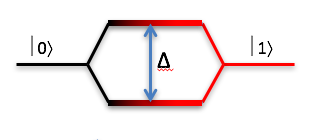
\includegraphics[height=4cm]{newSystem}
       \caption{\small The  original states  have the same  energy, but
         the superposition ones are split. \label{fig:newSystem}}
     \end{center}
   \end{figure}

   \textbf{Now  we add  an electric  field} to  the quantum  wells, see
   Fig.\ref{fig:withField}.   The  energy  shift   from  the  field  is
   $e\vec{E}\vec{d}$, where  $\vec{d}$ is the distance  between the two
   wells. We have a two level system,  and we define the zero energy to
   be halfway between them, making the Hamiltonian

   \begin{equation}
     \label{l1-1}
     \mathcal{H}_{\text{no tunneling}} = -\frac{\epsilon}{2}\sigma_z = \left(\begin{matrix}
         -\epsilon/2 & 0\\ 0 & \epsilon/2
       \end{matrix}\right).
   \end{equation}

   \begin{figure}
     \begin{center}
       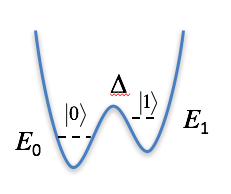
\includegraphics[height=3cm]{withField}
       \caption{\small  Adding an  electric field,  will mean  that one
         well state is at a higher energy (higher potential energy).}
       \label{fig:withField}
     \end{center}
   \end{figure}

   \textbf{Now tunnelling + electric field gives us }

   \begin{equation}
     \begin{aligned}
       \mathcal{H}  =  \left(\begin{matrix}  -\epsilon/2   &  0\\  0  &
           \epsilon/2
         \end{matrix}\right) + \begin{pmatrix}
         0 & -\Delta/2\\-\Delta/2 & 0
       \end{pmatrix} & = {-\frac{\epsilon}{2}\sigma_z-\frac{\Delta}{2}\sigma_x}\\
       & = -\frac{\sqrt{\epsilon^2+\Delta^2}}{2}\left(\frac{\epsilon}{\sqrt{\epsilon^2+\Delta^2}}\sigma_z+\frac{\Delta}{\sqrt{\epsilon^2+\Delta^2}}\sigma_x\right)\\
       & = -\frac{\Delta E}{2}\left(\cos\left(\theta\right)\sigma_z+\sin\left(\theta\right)\sigma_x\right)\\
       \red{\Rightarrow     \left\lbrace\begin{aligned}    \mathcal{H}     &    =
             \mathbf{-\frac{\Delta     E}{2}\begin{pmatrix}    \cos(\theta)     &
                 \sin(\theta)\\\sin(\theta) & -\cos(\theta)
               \end{pmatrix}}\\
             \Delta E & = \sqrt{\epsilon^2+\Delta^2}\\
             \tan(\theta) & = \frac{\Delta}{\epsilon}
           \end{aligned}\right.}
     \end{aligned},
   \end{equation}

   \noindent  \red{\text{ small  $\theta$ =  small mixing.}}.   Finding
   eigenvalues and eigenvectors

   \begin{equation}
     E = \pm \frac{\Delta E}{2}, \qquad \ket{\psi}_0 = \begin{pmatrix}
       \cos(\theta/2) \\ \sin(\theta/2)
     \end{pmatrix},  \qquad  \ket{\psi}_1  = \begin{pmatrix}  \sin(\theta/2)  \\
       -\cos(\theta/2)
     \end{pmatrix},
     \label{l1-finalEVal}
   \end{equation}

   \noindent and we note that  inside the Bloch Sphere, the eigenstates
   are now at an angle $\theta$ relative to the initial ``north-south''
   eigenstates as seen in Fig.\ref{newEigenstates}

   \begin{figure}[h]
     \begin{center}
       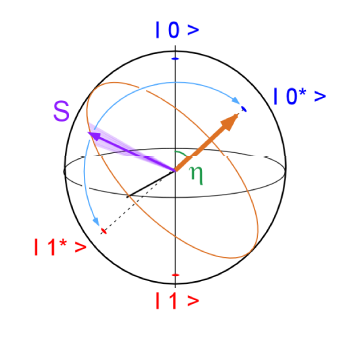
\includegraphics[height=4.5cm]{newEigenstates}
       \caption{\small The drive $\Delta$, tilts the eigenstates of the
         system. \red{$\tan(\theta) = \frac{\Delta}{\epsilon}$}}
       \label{newEigenstates}
     \end{center}
   \end{figure}

   \begin{framed}\noindent
     \noindent  So we  have gone  from a  purely potential  system with
     $\mathcal{H} =  -\epsilon/2\sigma_z$, and a purely  kinetic system
     with $\mathcal{H} = -\Delta/2\sigma_x$, to a mixed one as shown in
     Fig.\ref{l1-combined}.
   \end{framed}

   \begin{figure}[h]
     \begin{center}
       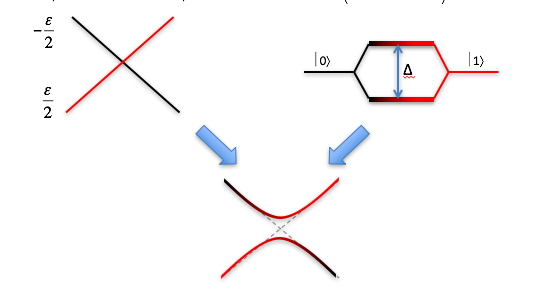
\includegraphics[height=7cm]{together}
       \caption{\small  In the  potential system,  the energies  of the
         eigenstates changed linearly with field. At the crossing point
         (no field), there is a degeneracy, where both wells are at the
         same  potential.  The  kinetic  tunnelling case  we have  also
         seen.  Together  they  form  a system  whose  eigenstates  are
         split.}
       \label{l1-combined}
     \end{center}
   \end{figure}


   \textbf{Considering      the       case      with       no      bias
     $\mathbf{\epsilon = 0 \Rightarrow \Delta E = \Delta, \theta = \pi/2}$:}

    \[
      \mathcal{H} = -\frac{\Delta}{2}
      \begin{pmatrix}
        0 & 1\\ 1 & 0
      \end{pmatrix} = -\frac{\Delta}{2} \sigma_x.
    \]

    \noindent Computing the unitary evolution of the state

    \begin{equation}
      \begin{aligned}
        U & = \exp\left[\frac{-i\mathcal{H}t}{\hbar}\right]\\
        & = \sum_k\frac{-i\Delta/2\sigma_xt}{k!}\\
        &    \red{=   \cos\left(\frac{\Delta}{2\hbar}t\right)\mathbb{I}    +
          i\sin\left(\frac{\Delta}{2\hbar}t\right)\sigma_x = \begin{pmatrix}
            \cos\left(\frac{\Delta}{2\hbar}t\right) & i\sin\left(\frac{\Delta}{2\hbar}t\right)\\
            i\sin\left(\frac{\Delta}{2\hbar}t\right)                       &
            \cos\left(\frac{\Delta}{2\hbar}t\right)
          \end{pmatrix}}
      \end{aligned},
      \label{l1-finalRot}
    \end{equation}

    \noindent so

   \begin{equation}
     U\ket{0} = \begin{pmatrix}
       \cos\left(\frac{\Delta}{2\hbar}t\right)\\
       i\sin\left(\frac{\Delta}{2\hbar}t\right),
     \end{pmatrix},
   \end{equation}

   \noindent so we can prepare any state perpendicular to the x-axis.

\begin{framed}\noindent
  Thus no bias + tunneling $ \equiv $  bias + resonant field in RWA. In both
  cases, the interaction causes the same state evolution
\end{framed}

\newpage
